% \documentclass[aspectratio=169,notes]{beamer}
\documentclass[aspectratio=169]{beamer}
\usetheme[faculty=phil]{fibeamer}
\usepackage{polyglossia}
\setmainlanguage{english} %% main locale instead of `english`, you
%% can typeset the presentation in either Czech or Slovak,
%% respectively.
\setotherlanguages{russian} %% The additional keys allow
%%
%%   \begin{otherlanguage}{czech}   ... \end{otherlanguage}
%%   \begin{otherlanguage}{slovak}  ... \end{otherlanguage}
%%
%% These macros specify information about the presentation
\title[Theoretical Mechanics]{Week HW 1, KIN PART ROT PLANE1} %% that will be typeset on the
\subtitle{ Particle kinematics \\
Rotational motion \\ Plane motion, simple \
         } %% title page.
\author{Oleg Bulichev}
%% These additional packages are used within the document:
\usepackage{ragged2e}  % `\justifying` text
\usepackage{booktabs}  % Tables
\usepackage{tabularx}
\usepackage{tikz}      % Diagrams
\usetikzlibrary{calc, shapes, backgrounds}
\usepackage{amsmath, amssymb}
\usepackage{url}       % `\url`s
\usepackage{listings}  % Code listings
% \usepackage{subfigure}
\usepackage{floatrow}
\usepackage{subcaption}
\usepackage{mathtools}
\usepackage{todonotes}
\usepackage{fontspec}
\usepackage{multicol}
\usepackage{pdfpages}
\usepackage{wrapfig}
\usepackage{animate}
\usepackage{booktabs}
\usepackage{multirow}
% \usepackage{graphicx}
\usepackage{colortbl}

\graphicspath{{resources/}}
\frenchspacing

\setbeamertemplate{caption}[numbered]
\usetikzlibrary{graphs}

% \usepackage[backend=biber,style=ieee,autocite=footnote]{biblatex}
% \addbibresource{biblio.bib}
% \DefineBibliographyStrings{english}{%
%   bibliography = {References},}

\newcommand{\oleg}[2][] {\todo[color=red, #1] {OLEG:\\ #2}}
\newcommand{\fbckg}[1]{\usebackgroundtemplate{\includegraphics[width=\paperwidth]{#1}}}%frame background

\usepackage[framemethod=TikZ]{mdframed}
\newcommand{\dbox}[1]{
\begin{mdframed}[roundcorner=3pt, backgroundcolor=yellow, linewidth=0]
\vspace{1mm}
{#1}
\vspace{1mm}
\end{mdframed}
}

\begin{document}
\setlength{\abovedisplayskip}{0pt}
\setlength{\belowdisplayskip}{0pt}
\setlength{\abovedisplayshortskip}{0pt}
\setlength{\belowdisplayshortskip}{0pt}

\fbckg{fibeamer/figs/title_page.png}
\frame[c]{\setcounter{framenumber}{0}
    \usebeamerfont{title}%
    \usebeamercolor[fg]{title}%
    \begin{minipage}[b][6.5\baselineskip][b]{\textwidth}%
        \textcolor{black}{\raggedright\inserttitle}
    \end{minipage}
    % \vskip-1.5\baselineskip

    \usebeamerfont{subtitle}%
    \usebeamercolor[fg]{framesubtitle}%
    \begin{minipage}[b][3\baselineskip][b]{\textwidth}
        \raggedright%
        \insertsubtitle%
    \end{minipage}
    \vskip.25\baselineskip
}
%   \frame[c]{\maketitle}

\fbckg{fibeamer/figs/common.png}

\section*{Formal rules}

\begin{frame}[t]{Week HWs formal rules}
    \framesubtitle{Grading}
    \begin{enumerate}
        \footnotesize
        \item HW costs 5 point max.
        \item Not late policy. If you submit it later, 0 points.
        \item Score distribution:
        \begin{itemize}
            \footnotesize
            \item Correct formal criteria and document structure --- 1 score.
            \item Correct algorithm and idea --- 2 out of 5 for sure.
            \item Correct plots and simulation --- 2 out of 5.
        \end{itemize}
    \end{enumerate}
    \end{frame}

\begin{frame}[t]{Week HWs formal rules}
\framesubtitle{Tasks and formal reporting}
\textbf{Tasks}
\begin{enumerate}
    \footnotesize
    \item If task has label "coding", it should be not only solved, but also coded.
    \item It's a good practice to code not coding task, for checking your calculations (not obligatory).
    \item Consider, that this report you are making for yourself to use it in future. I mean, it can be helpful sometimes to put full solution, not like "(1) eqn -> after trivial magical passes (2)". It's recommended to explain each step (it helps you and me to find mistakes and typos).
    \item Each HW is a report. It consists of a solution (don't forget about formal criteria), info about tools which were used, link to the code.
\end{enumerate}
\textbf{Formal reporting}
\begin{enumerate}
    \footnotesize
    \item In Moodle you are sending only a report (other stuff are links). \textbf{IN PDF}, \textit{txt} files won't be opened.
    \item We are in IT university, hence it's obligatory that your code should work on other computers.
\end{enumerate}
\end{frame}

    \begin{frame}[t]{Week HWs formal rules}
    \framesubtitle{Report template}
        \begin{enumerate}
            \footnotesize
            \item \textbf{Tools}. Write, what tools did you use for solving task (Python/Matlab ..., Latex/Markdown ...)
            \item \textbf{Link to the simulation}. If you put report together with the code, then the path is needed.
            \item \textbf{Task description}. Retype or put a screenshot of the task.
            \item \textbf{Task explanation}. It can be typed or be handwritten, or mixed. The goal, to explain step by step, how did you solve the task. You should explain your formulas too.

            I'd like to highlight, that the way how do you make a simulation is also worthy for be explained.

            Assume, that you are writing it for yourself, and you will read it later.
            \item \textbf{Plots}. Put needed plots. Don't forget to make an appropriate title, legend, and axes description.
            \item \textbf{Screenshots from simulation}. Several screenshots, in some interesting positions. Example: parabola --- midway of left branch, root, somewhere in right branch.
            \item \textbf{Meme (optional)}. Put funny picture/video))
        \end{enumerate}
    \end{frame}

    \begin{frame}[t]{Simulation examples}
    \framesubtitle{}
        \begin{figure}[H]
            \begin{subfigure}{0.32\textwidth}
                \centering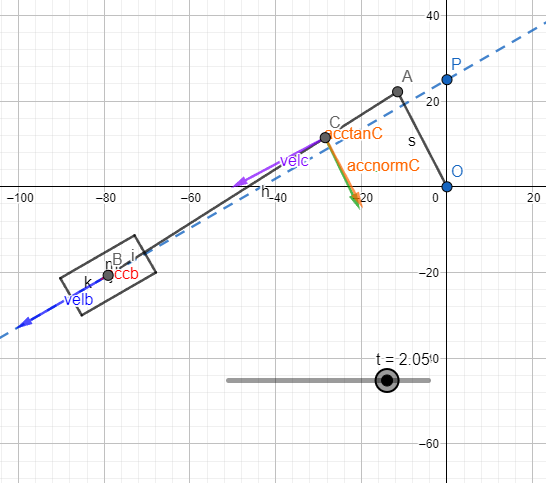
\includegraphics[height=6cm,width=1\textwidth,keepaspectratio]{geo.png}
                \caption{\href{https://www.geogebra.org/}{Geogebra app}}
                \label{fig:geo.png}
            \end{subfigure}
            \begin{subfigure}{0.32\textwidth}
                \centering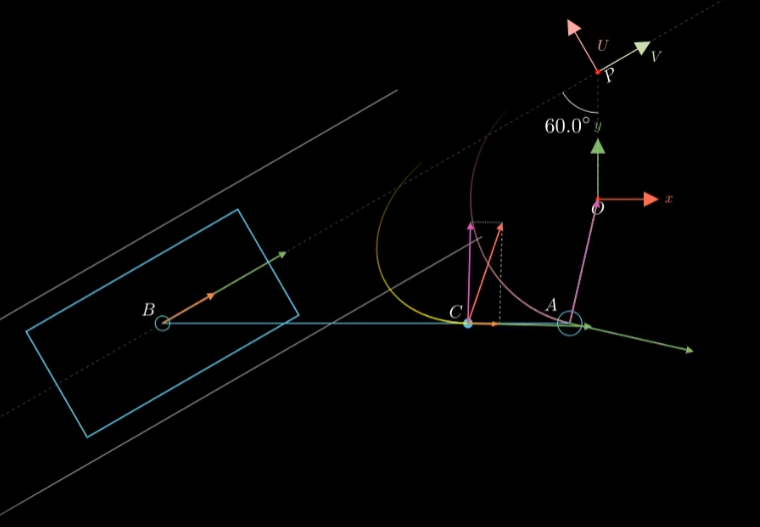
\includegraphics[height=6cm,width=1\textwidth,keepaspectratio]{manim.png}
                \caption{\href{https://www.manim.community/}{Manim library}}
                \label{fig:manim.png}
            \end{subfigure}
            \begin{subfigure}{0.32\textwidth}
                \centering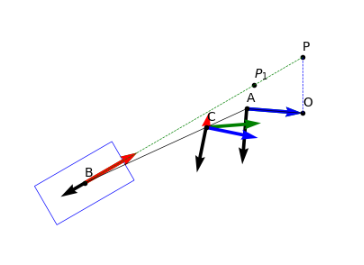
\includegraphics[height=6cm,width=1\textwidth,keepaspectratio]{matplotlib.png}
                \caption{\href{https://matplotlib.org/stable/users/explain/animations/animations.html\#sphx-glr-users-explain-animations-animations-py}{Matplotlib animations}}
                \label{fig:matplotlib.png}
            \end{subfigure}
        
        \caption*{Code samples: \href{https://colab.research.google.com/drive/10qiTOlywP5XTFUXQ-549huNInDtRE1NT?usp=sharing}{Here}}
        \end{figure}
    \end{frame}

    \section*{Tasks}

\begin{frame}[t]{Task 1 (Coding)}
\begin{minipage}{0.49\textwidth}

    
    You should find:
    \begin{enumerate}
        \item simulate the move of $\vec{O}$ for $t=[0..10]$;
        \item find and draw plots $v,\ a,\ a_n,\ a_\tau,\ \kappa $ (Osculating circle) respect to $t$;
        \item find  $y(x)$, $\vec{v}$, $\vec{a}$, $\vec{a}_n$, $\vec{a}_\tau$ and show it on the simulation.
    \end{enumerate}
    \end{minipage}
    \begin{minipage}{0.49\textwidth}
    \begin{equation*}
        \vec{O} = \left\{\begin{matrix}x = 3\cos(2t)\cos(t)+0.82\\y = 3\cos(2t)\sin(t)+0.82
        \end{matrix}\right.
    \end{equation*}
    \end{minipage}
\end{frame}

\begin{frame}[t]{Task 2 (Coding)}
    \vspace*{-0.2cm}
\begin{minipage}{0.6\textwidth}
    You should solve the task, till the $M$ point travels $s$:
    \begin{enumerate}
        \item simulate this mechanism (obtain all positions of bodies 1, 2, 3)
        \item velocity for $M$(draw plots for magnitudes and show vectors on simulation);
        \item accelerations (tangent, normal, overall) for $M$(draw plots for magnitudes and show vectors on simulation);
        \item draw plots of angular velocities for $2,\ 3$ bodies.
    \end{enumerate}
    If $R_2=40,\ r_2=30,\ R_3=15$\\ 
    $x=x(t)=3+80t^2,\ s_M=4$.
    
    \end{minipage}
    \begin{minipage}{0.39\textwidth}
          \begin{figure}[H]
        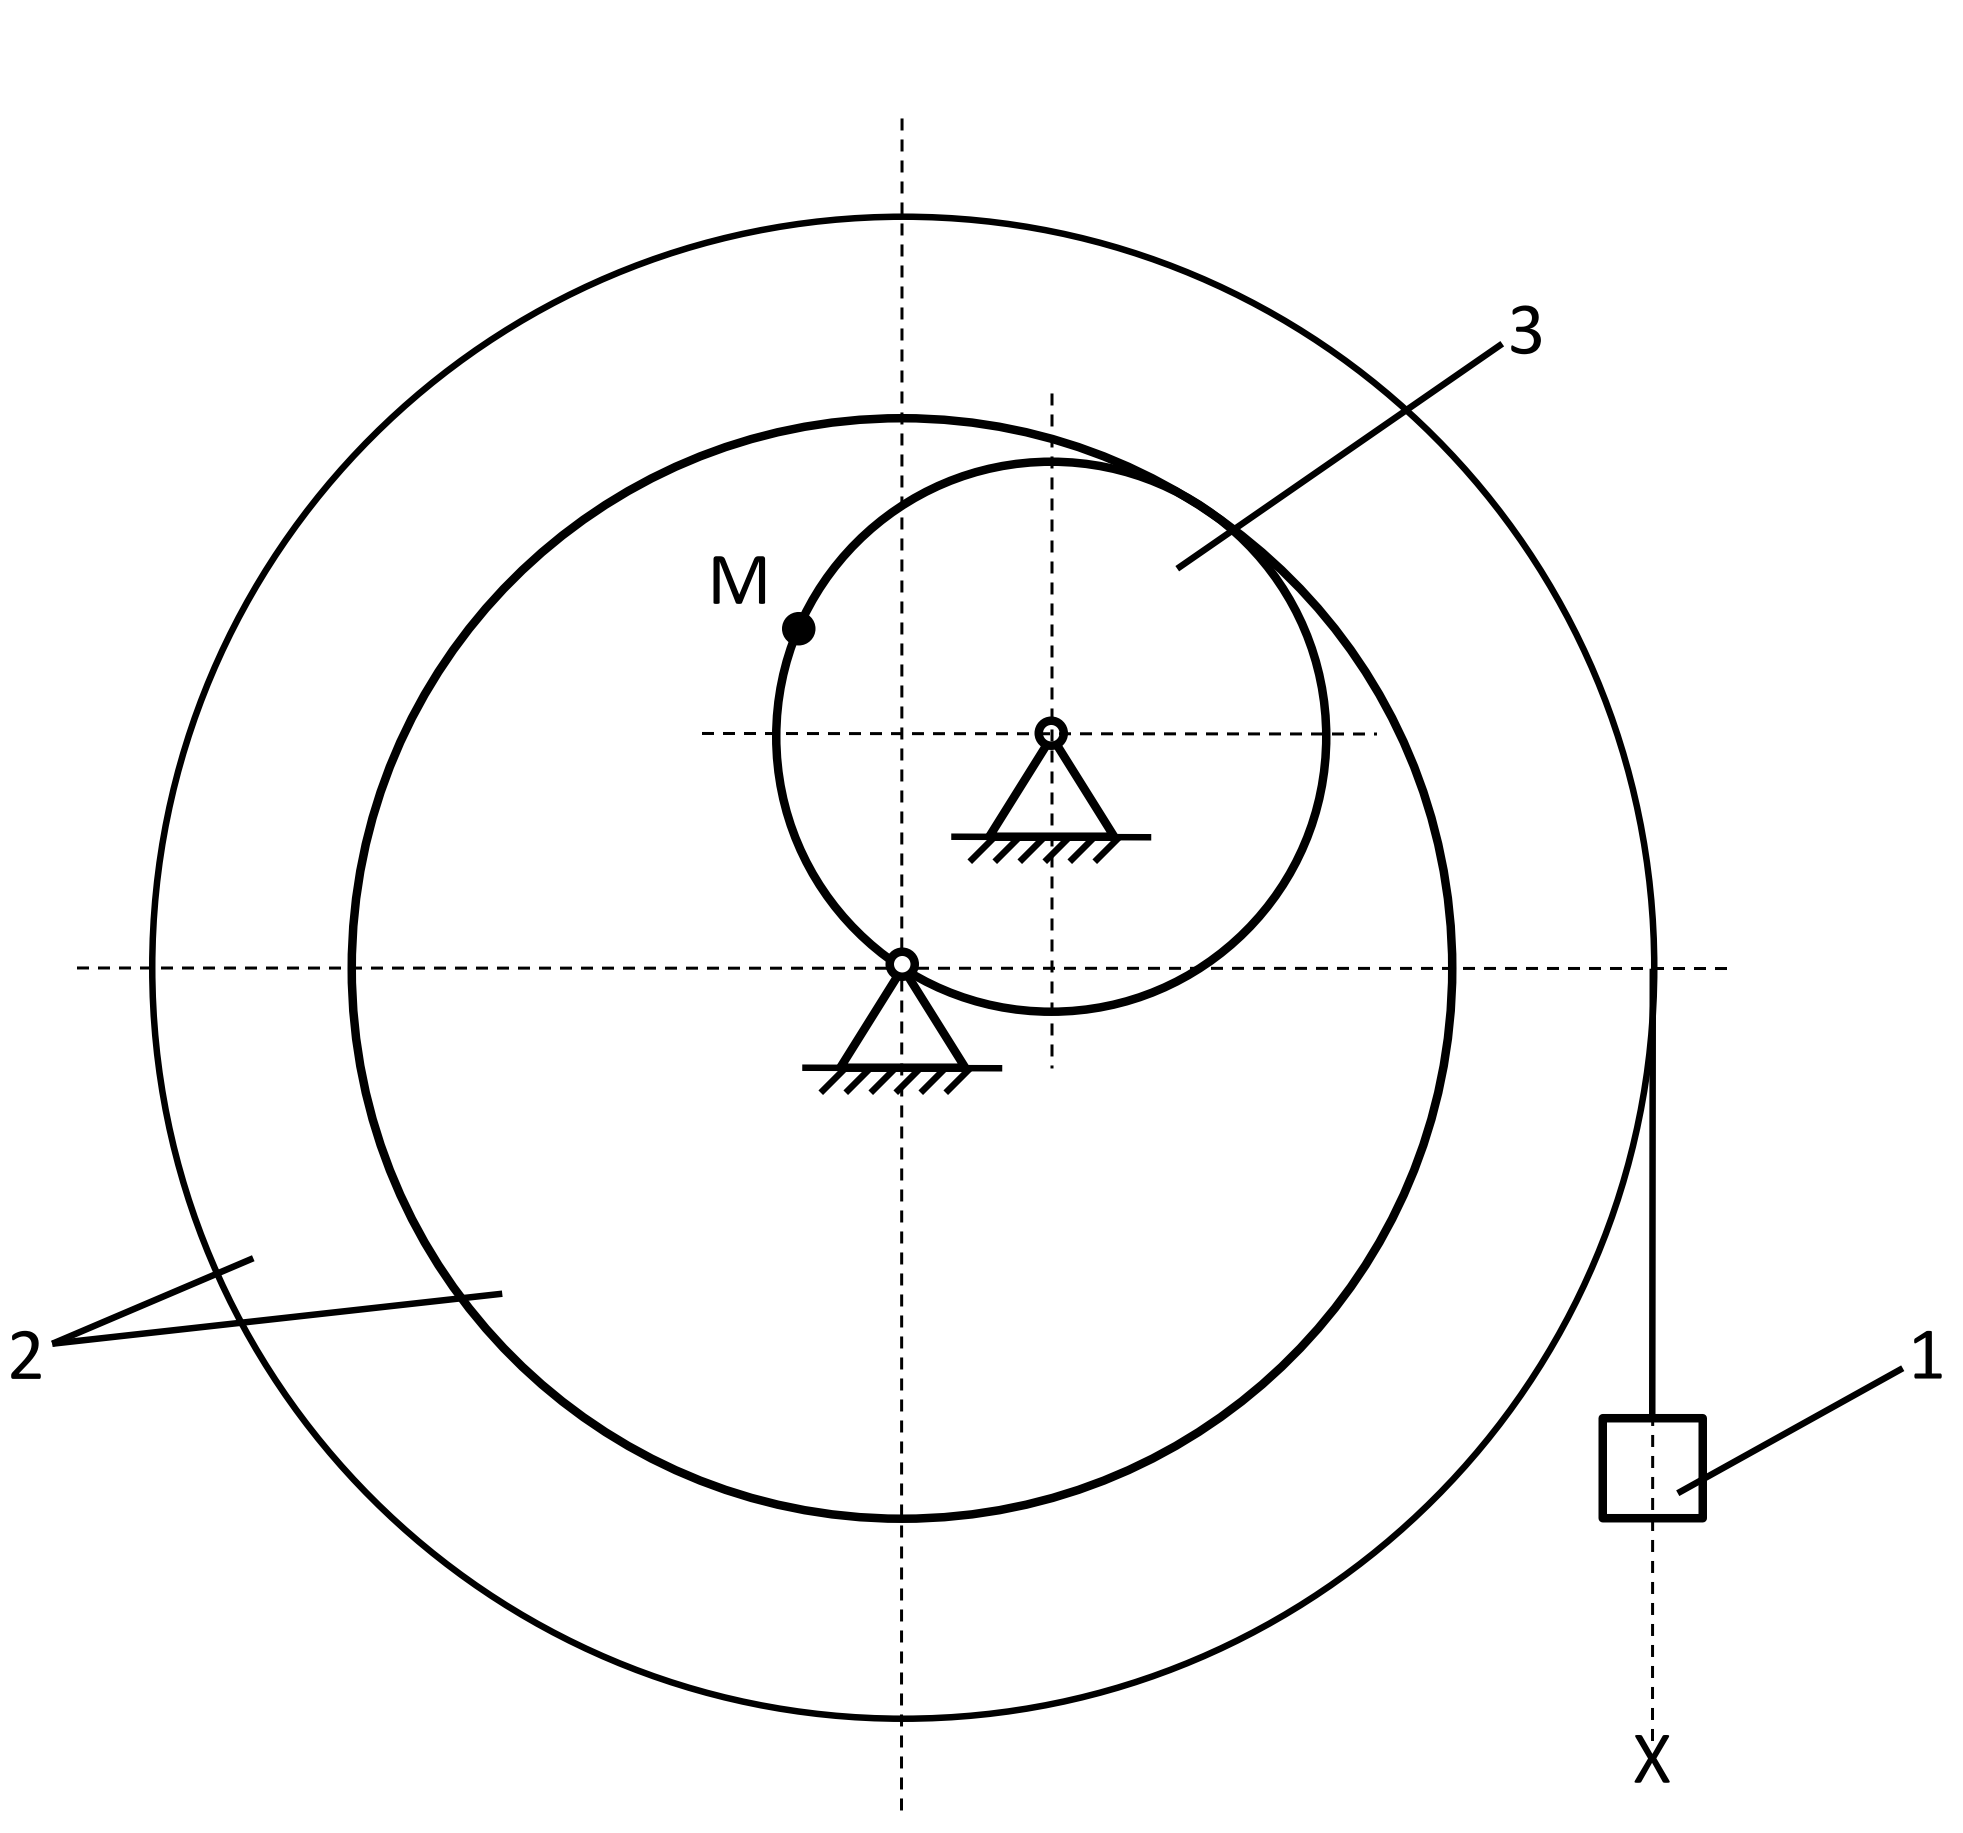
\includegraphics[width=0.99\textwidth]{HW1_2.png}
        \caption*{Task 2 \\ (Yablonskii (eng) K2}
        \end{figure}
    \end{minipage}
\end{frame}


\begin{frame}[t]{Task 3 (Coding)}
    \begin{minipage}{0.6\textwidth}
        You should find:
        \begin{enumerate}
            \item simulate this mechanism (obtain all positions.) ($x_i(t),\ y_i(t)$, where $i$ is $A,\ B,\ C$ point)
            \item velocities for $B,\ C$ (draw plots for magnitudes and show vectors on simulation);
            \item accelerations for $B$ and $C$ (draw plots for magnitudes and show vectors on simulation);
            \item draw a plot of angular velocity of body $BA$.
        \end{enumerate}
        If $ y_A(t)=22.5+10sin(\frac{\pi}{5}t);\ t = [0..10]\ sec.;\\ AB=45,\ BC=30$.  \\
        \end{minipage}
        \begin{minipage}{0.39\textwidth}
            \vspace{-0.2cm}
              \begin{figure}[H]
            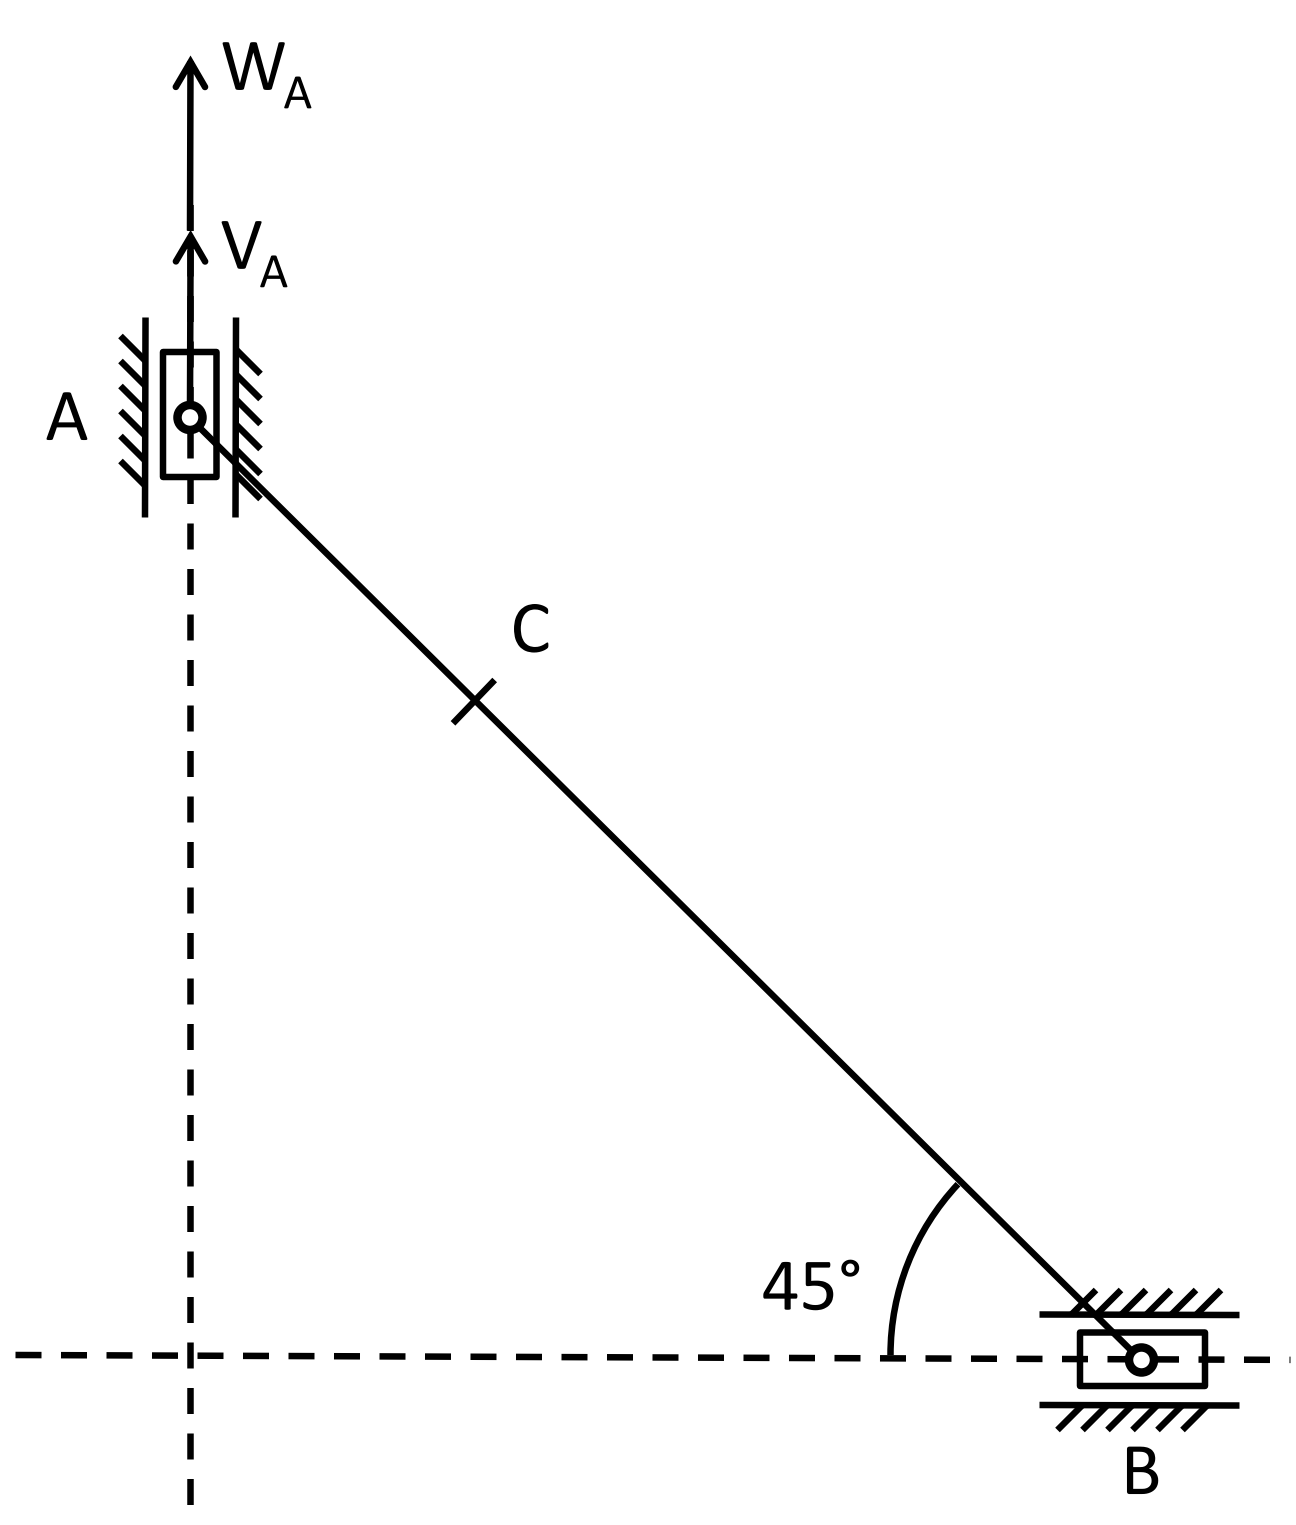
\includegraphics[height=5cm, width=0.99\textwidth, keepaspectratio]{HW1_3.png}\\
            \caption*{Task 3 \\ (Yablonskii (rus) K3)}
            \end{figure}
        \end{minipage}
\end{frame}

\fbckg{fibeamer/figs/last_page.png}
\frame[plain]{}
\end{document}